\documentclass[titlepage = firstcover]{scrartcl}
\usepackage[aux]{rerunfilecheck}
\usepackage{fontspec}
\usepackage[main=ngerman, english, french]{babel}

% mehr Pakete hier
\usepackage{expl3}
\usepackage{xparse}

%Mathematik------------------------------------------------------
\usepackage{amsmath}   % unverzichtbare Mathe-Befehle
\usepackage{amssymb}   % viele Mathe-Symbole
\usepackage{mathtools} % Erweiterungen für amsmath
\usepackage[
  math-style=ISO,    % \
  bold-style=ISO,    % |
  sans-style=italic, % | ISO-Standard folgen
  nabla=upright,     % |
  partial=upright,   % /
]{unicode-math}% "Does exactly what it says on the tin."
\usepackage[section, below]{placeins}

% Laden von OTF-Mathefonts
% Ermöglich Unicode Eingabe von Zeichen: α statt \alpha

\setmathfont{Latin Modern Math}
%\setmathfont{Tex Gyre Pagella Math} % alternativ zu Latin Modern Math
\setmathfont{XITS Math}[range={scr, bfscr}]
\setmathfont{XITS Math}[range={cal, bfcal}, StylisticSet=1]

\AtBeginDocument{ % wird bei \begin{document}
  % werden sonst wieder von unicode-math überschrieben
  \RenewDocumentCommand \Re {} {\operatorname{Re}}
  \RenewDocumentCommand \Im {} {\operatorname{Im}}
}
\usepackage{mleftright}
\setlength{\delimitershortfall}{-1sp}

%Sprache----------------------------------------------------------
\usepackage{microtype}
\usepackage{xfrac}
\usepackage[autostyle]{csquotes}    % babel
\usepackage[unicode, pdfusetitle]{hyperref}
\usepackage{bookmark}
\usepackage[shortcuts]{extdash}
%Einstellungen hier, z.B. Fonts
\usepackage{booktabs} % Tabellen


\title{Brückenschaltungen}
\author{
  David Gutnikov\\
  \href{mailto:david.gutnikov@udo.edu}{david.gutnikov@udo.edu}
 \and 
  Lasse Sternemann\\
  \href{mailto:lasse.sternemann@udo.edu}{lasse.sternemann@udo.edu}
}
\date{Durchführung am 03.12.2019}

\begin{document}
    \maketitle
    \tableofcontents
    \newpage

    \section{Zielsetzung}
        Mithilfe von verschiedenen Brückenschaltungen sollen elektrische Widerstände und die damit verbundenen physikalischen Größen, wie z.B. die Kapazität
        eines Kondensators oder die Induktivität einer Spule, möglichst genau gemessen werden.



    \section{Theoretische Grundlagen}
        \subsection{Allgemeine Brückenschaltung}
          Brückenschaltungen bestehen aus vier oder mehr Widerständen, die wie in Abbildung \ref{fig:brueckenschalt} parallel und dann in Reihe geschaltet
          sind.
          \begin{figure}[h]
            \centering
            \caption{Die Abbildung einer einfachen Brückenschaltung.}
            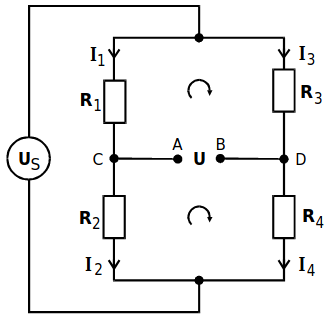
\includegraphics[width = 0.4\linewidth]{Brueckenschaltung.png}
            \label{fig:brueckenschalt}
          \end{figure}
      
          \FloatBarrier
          \noindent
          Hierbei wird die Spannung zwischen den Punkten A und B, als Brückenspannung $U$ bezeichnet. Diese Spannung lässt sich mit Hilfe der Kirchhoffschen
          Gesetze durch die bekannten Größen der Widerstände und der Speisespannung $U_S$ darstellen.
          Die Kirchhoffschen Gesetze lauten:
          \subsubsection{Knotenregel}
            In jedem Knotenpunkt in dem sich elektrische Ströme verzweigen, ist die Summe der hineinfließenden und der herausfließenden Ströme gleich.
            \begin{equation}
              I_1 = I_2 + I_3
            \end{equation}
            \begin{figure}[h]
              \centering
              \caption{Das Beispiel eines Verzweigungspunktes el. Ströme.}
              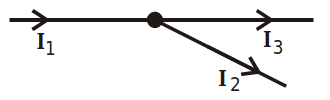
\includegraphics[width = 0.4\linewidth]{Kirchhoff_1.png}
              \label{fig:kirchhoff1}
            \end{figure}
            \FloatBarrier

          \subsubsection{Maschenregel}
            Alle Teilspannungen einer Masche eines elektrischen Netzwerkes summieren sich zu null. Dabei legt man eine Zählrichtung fest (meistens im Uhrzeigersinn). Zeigt der Strom
            an den Teilspannungen in Zählrichtung, so wird diese positiv gezählt ($I_k > 0$), zeigt er in die entgegengesetzte Richtung, kriegt die Teilspannung ein negatives
            Vorzeichen ($I_k < 0$).
            \begin{equation}
              \sum_k E_k = \sum_k I_k \cdot R_k
            \end{equation}
            \begin{figure}[h]
              \centering
              \caption{Das Beispiel einer Masche in einem Stromnetzwerk.}
              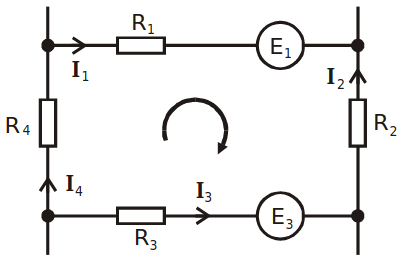
\includegraphics[width = 0.4\linewidth]{Kirchhoff_2.png}
              \label{fig:kirchhoff2}
            \end{figure}
            \FloatBarrier

          Somit sähe die Brückenspannung wie folgt aus:
          \begin{equation}
            \label{eqn:brueckspannung}
            U = \frac{R_2 R_3 - R_1 R_4}{(R_3 + R_4) (R_1 + R_2)}U_S
          \end{equation}
          Da hier jedoch die Nullmethode angewendet wird muss $U = 0$ sein. Das wird durch folgendes Verhältnis erreicht wie in \eqref{eqn:brueckspannung}
          leicht zu erkennen ist:
          \begin{equation}
            \label{eqn:abgleichbed}
            R_1 R_4 = R_2 R_3
          \end{equation}
          Da diese Abgleichbedingung nur von den Verhältnissen der Widerstände abhängt wird diese Brückenschaltung "abgeglichene Brücke" genannt und es ist
          möglich eine Widerstandsmessung durchzuführen mit drei bekannten Widerständen.

        \subsection{Brückenschaltung mit komplexen Widerständen}
          Es ist auch möglich Kapazitäten und Iduktivitäten in eine Brückenschaltung mit einzubauen, dabei ist es sinnvoll kompelexe Widerstände zu benutzen,
          welche allgemein wie folgt aussehen:
          \begin{equation}
            \label{eqn:komplexwiderstand}
            R_Z = X + \text{i} Y
          \end{equation}
          Damit würde eine Brückenschaltung mit vier komplexen Widerständen folgende Abgleichbedingung nach \eqref{eqn:abgleichbed} haben:
          \begin{align}
            R_{Z1} R_{Z4} &= R_{Z2} R_{Z3} \\
            (X_1 + \text{i} Y_1)(X_4 + \text{i} Y_4) &= (X_2 + \text{i} Y_2)(X_3 + \text{i} Y_3)
          \end{align}
          Durch das Gleichstellen der Real- und Imaginärteile entstehen zwei Bedingungen:
          \begin{align}
            \label{eqn:komplexabgleich1}
            X_1 X_4 - Y_1 Y_4 &= X_2 X_3 - Y_2 Y_3 \\
            \label{eqn:komplexabgleich2}
            X_1 Y_4 + X_4 Y_1 &= X_2 Y_3 + X_3 Y_2
          \end{align}
          Beide Bedingungen müssen also bei einer Wechselstrombrücke erfüllt sein. Die Brückenspannung muss im Betrag verschwinden, dabei muss noch die Phase
          ausgeglichen werden. Deshalb muss jede Wechselstrombrücke zwei unabhängige, veränderliche Stellglieder haben.

        \subsection{Wheatstonesche Brücke}
          Mit der Wheatstoneschen Brücke werden Widerstände gemessen. Sie ist in Abbildung \ref{fig:wheatstone} dargestellt.
          \begin{figure}[h]
            \centering
            \caption{Die Wheatstonesche Brücke zur Widerstandsmessung.}
            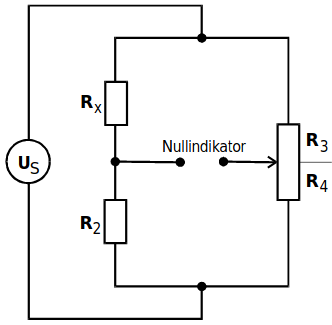
\includegraphics[width = 0.4\linewidth]{Wheatstoneschebruecke.png}
            \label{fig:wheatstone}
          \end{figure}
          Der gesuchte Widerstand $R_X$ wird durch Formel \eqref{eqn:abgleichbed} berechnet:
          \begin{equation}
            \label{eqn:abgleichbed}
            R_X = R_2 \frac{R_3}{R_4}
          \end{equation}

        \subsection{Kapazitätsmessbrücke}
          Da es keine idealen Kondensatoren in der Realität gibt, d.h. jeder reale Kondensator wandelt einen kleinen Teil der el. Energie in Wärme um,
          werden Kondensatoren durch Ersatzschaltbilder, als ein in Reihe geschalteter Widerstand R und idealer Kondensator mit der Kapazität $C$ dargestellt.
          Somit sieht der komplexe Widerstand des realen Kondesators wie folgt aus:
          \begin{equation}
            R_C = R - \text{i} \frac{1}{\omega C}
          \end{equation}
          Es gibt also zwei Unbekannte, den Widerstand $R_X$ und die Kapazität $C_X$. Deshalb werden auch zwei Abstimmffreiheitsgrade gebraucht, um der
          Phasenverschiebung aufgrund von $R_X$ entgegenzuwirken. Hier wird dazu der Widerstand $R_2$ verändert.
          \begin{figure}[h]
            \centering
            \caption{Die Kapazitätsmessbrücke.}
            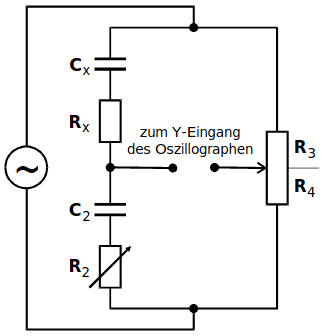
\includegraphics[width = 0.4\linewidth]{Kapazitaetsmessbruecke.png}
            \label{fig:wheatstone}
          \end{figure}
          Es gelten für diese Schaltung nach \eqref{eqn:komplexwiderstand}
          \begin{align*}
            &X_1 = R_X, & X_2 &= R_2, & X_3 =& R_3, & X_4 =& R_4 \\
            &Y_1 = -\frac{1}{\omega C_X}, & Y_2 &= -\frac{1}{\omega C_2}, & Y_3 =& 0, & Y_4 =& 0
          \end{align*}
          Das wird in \eqref{eqn:komplexabgleich1} und \eqref{eqn:komplexabgleich2} eingesetzt und nach den gesuchten Größen umgestellt:
          \begin{align}
            R_X = R_2 \frac{R_3}{R_4} &&\text{und}&& C_X = C_2 \frac{R_4}{R_3}            
          \end{align}

          \subsection{Induktivitätsmessbrücke}
          Auch hier gibt es keine ideale Spule in der Realität. An jeder realen Spule existiert ein Spannungsabfall, deshalb wird hier genauso wie bei den
          Kondensatoren verfahren und die Spulen werden, als ein in Reihe geschalteter Widerstand R und ideale Spule mit Induktivität $L$ dargestellt. 
          \begin{equation}
            R_C = R - \text{i} \omega L
          \end{equation}
          Es gibt wieder zwei Unbekannte, den Widerstand $R_X$ und die Induktivität $L_X$. Deshalb werden auch zwei Abstimmfreiheitsgrade gebraucht, um der
          Phasenverschiebung aufgrund von $R_X$ entgegenzuwirken. Hier wird wie bei der Kapazitätsmessung der Widerstand $R_2$ verändert.
          \begin{figure}[h]
            \centering
            \caption{Die Induktivitätsmessbrücke.}
            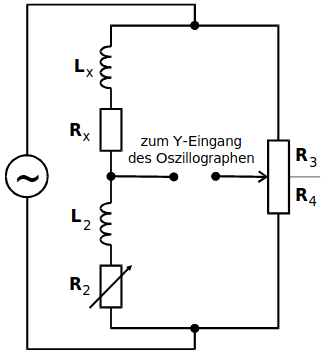
\includegraphics[width = 0.4\linewidth]{Induktivitaetsmessbruecke.png}
            \label{fig:wheatstone}
          \end{figure}
          Es gelten für diese Schaltung nach \eqref{eqn:komplexwiderstand}
          \begin{align*}
            &X_1 = R_X, & X_2 &= R_2, & X_3 =& R_3, & X_4 =& R_4 \\
            &Y_1 = \text{i} \omega L_X, & Y_2 &= \text{i} \omega L_2, & Y_3 =& 0, & Y_4 =& 0
          \end{align*}
          Nach dem gleichen Muster wie bei der Kapazitätsmessbrücke wird auch hier verfahren und es kommen ähnliche Formeln als Ergebnisse heraus:
          \begin{align}
            R_X = R_2 \frac{R_3}{R_4} &&\text{und}&& L_X = L_2 \frac{R_3}{R_4}            
          \end{align}
          Allerdings sollten die Verluste an der Spule mit der Induktivität $L_2$ bei dieser Methode sehr klein sein, was im Gegensatz zu einem verlustarmen
          Kondensator schwierig zu realisieren ist. Deshalb wird die Spule in einer anderen Schaltung durch einen Kondensator ersetzt. Diese Schaltung für die
          Induktionsmessung wird Maxwell-Brücke genannt.
        \FloatBarrier

        \newpage

        \subsection{Maxwell-Brücke}
          Auch hier sind die Widerstände $R_3$ und $R_4$ veränderbar.
          \begin{figure}[h]
            \centering
            \caption{Die Maxwell-Brücke zur Induktivitätsmessung.}
            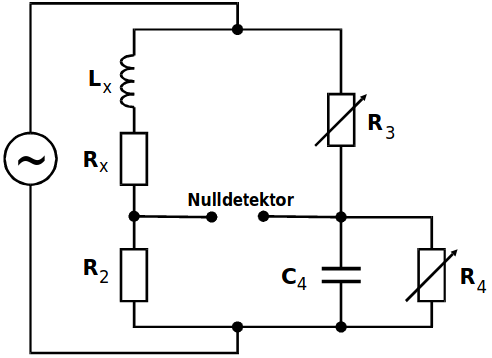
\includegraphics[width = 0.5\linewidth]{Maxwellbruecke.png}
            \label{fig:maxwellbr}
          \end{figure}
          Und die zwei Abgleichbedingungen, welche man nach dem gleichen Vorgehen wie davor kriegt, lauten
          \begin{align}
            R_X = R_2 \frac{R_2 R_3}{R_4} &&\text{und}&& L_X = R_2 R_3 C_4             
          \end{align}
          \FloatBarrier

      \noindent
      Die bisher vorgestellten Brückenschaltungen waren frequenzunabhängig. Nur für die praktischen Zwecke war es günstig keine zu hohe Frequenz zu wählen,
      da sonst der Einfluss der Streukapazitäten zu sehr in die Messung eingehen würde und keine zu niedrigen Frequenzen zu wählen, da es ein paar
      Einschwingvorgänge braucht bevor sich eine für die Messung brauchbare stationäre Brückenspannung einpendelt.

        \subsection{Wien-Robinson-Brücke}
          Diese Brücke besitzt keine variierbaren Elemente zum Abgleich. Stattdessen wird die Speisespannung verändert, so dass sich eine möglichst
          kleine Brückenspannung ergibt.
          \begin{figure}[h]
            \centering
            \caption{Die Wien-Robinson-Brücke zum Frequenzfiltern.}
            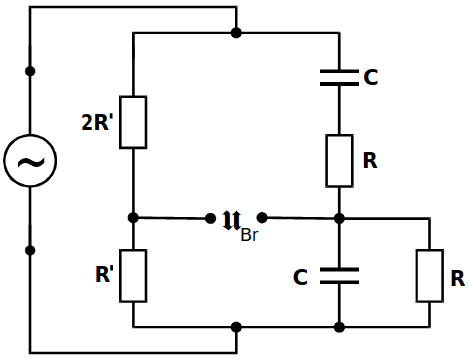
\includegraphics[width = 0.4\linewidth]{Wien_Robinson.png}
            \label{fig:wienrobinsonbr}
          \end{figure}
          \FloatBarrier
          \noindent
          Durch ähnliche Überlegungen wie bei den vorherigen Brückenschaltungen erschließt sich ein Verhältnis von Brückenspannung $U_Br$ zur
          Speisespannung $U_S$:
          \begin{equation}
            \label{eqn:wienrob}
            \biggl(\frac{U_{Br}}{U_S} \biggr)^2 = \frac{\bigl(\omega^2 R^2 C^2 - 1 \bigr)^2}{9\Bigl(\bigl(1 - \omega^2 R^2 C^2 \bigr)^2 + 9 \omega^2 R^2 C^2 \Bigr)}
          \end{equation}
          Es ist deutlich, dass dieser Ausdruck wenn gilt
          \begin{equation*}
            \omega_0 = \frac{1}{R C}
          \end{equation*}
          Zur besseren Einsehbarkeit wird das folgende Verhältnis eingeführt
          \begin{equation*}
            \Omega = \frac{\omega}{\omega_0}
          \end{equation*}
          Mit den beiden oberen Formeln wird \eqref{eqn:wienrob} zu
          \begin{equation}
            \label{eqn:wienrob}
            \biggl(\frac{U_{Br}}{U_S} \biggr)^2 = \frac{1}{9} \frac{\bigl(\Omega^2 - 1 \bigr)^2}{\bigl(1 - \Omega^2 \bigr)^2 + 9 \Omega^2}
          \end{equation}
          Es wird klar, dass die Wien-Robinson-Brücke als Frequenzfilter fungiert, welcher die Frequenz $\omega_0$ aus dem Frequenzspektrum filtert und
          die umliegenden Frequenzen stark abschwächt.
\end{document}